\section{Актуальность темы}
\begin{frame}
    {Актуальность темы}
    
    В настоящее время тенденция бурного развития информационных технологий во всех сферах деятельности человека оказывает весомое влияние на нефтегазовый сектор страны. Соврменные компании, представляющие собой сложные многоуровневые производственные системы, для своего устойчивого развития требуют постоянного развития информационных технологий.  
    \bigskip

    Сегодня наблюдается  бурное развитие процесса «цифровизации» нефтегазовой отрасли. Одним из путей развития данного процесса является внедрение беспроводных технологий.
    
    
\end{frame}

\begin{frame}
    {Актуальность темы}
    Активное использование беспроводных сетей основывается на ряде их преимуществ по сравнению с кабельными сетями:
    \begin{itemize}
        \item возможность получения информации с любой точки контролируемой территории;
        \item быстрый ввод в эксплуатацию по системе подключение типа Plug-\&-Play;
        \item сокращение капитальных затрат на создание сети; 
        \item уменьшение затрат на эксплуатацию;
        \item высокая гибкость, мобильность, масштабируемость;
        \item упрощенные требования к обслуживанию оборудования.
    \end{itemize}

  
\end{frame}

\section{Научно-техническая проблема}
\begin{frame}
    {Научно-техническая проблема}

    В рамках этого процесса возникает актуальная научно - техническая проблема \textbf{повышения качества проектирования беспроводной сети связи}, осуществляющей сбор и передачу информации в центр  управления с множества контролируемых объектов на некоторой территории. 

\end{frame}


\begin{frame}
    {Научно-техническая проблема}
    Процесс проектирования енной беспроводных сетей связи (БШС) состоит из последовательного решения взаимосвязанных задач:
    
    \bigskip

    \begin{itemize}
        \item выбор типов технических средств и протоколов;
        \item выбор топологической структуры сети;
        \item анализ и оптимизация пропускной способности каналов связи, маршрутизация информационных потоков и др.
    \end{itemize}

    \bigskip
    
    Задача \textbf{синтеза топологии} при комплексном проектировании БШС является основной проблемой исследования в данной работе.

\end{frame}

\begin{frame}
    {Научно-техническая проблема}

    \textbf{\underline{Объектом исследования}} БШС специальных типов, широко представленных на практике:
    
    \bigskip

    \begin{itemize}
        \item БШС для контроля линейных траекторий;
        \item БШС с ячеистой топологией (mesh) для контроля объектов, рассредоточенных на некоторой территории.
    \end{itemize}

    \bigskip

    \textbf{\underline{Предметом исследования}} является синтез топологической структуры беспроводной широкополосной сети.

    \bigskip
    
    \textbf{\underline{Целью}} состоит в разработке моделей и методов оптимального размещения базовых станций для БШС указанных типов, определяющего топологию таких сетей.
\end{frame}

\section{Положение 1}
\begin{frame}
    \begin{center}
        {Положение 1 - математические модели в виде задачи ЦЛП и экстремальной комбинаторной задачи для оптимального размещения базовых станций при проектировании БШС с линейной топологией}
    \end{center}
\end{frame}

\begin{frame}
    {Технологическая постановка задачи} 

    Для контроля над заданным линейным участком необходимо разместить базовые приемопередающие устройства (станции) таким образом, чтобы максимизировать покрытие с обеспечением условий технических и бюджетных ограничений. 

    \bigskip
    
    Постановка
    \begin{itemize}
        \item в виде задачи ЦЛП;
        \item в виде комбинаторной модели в экстремальной форме.
    \end{itemize}

\end{frame}

% \begin{frame}
%     Важно обеспечить связь любой станции со шлюзами на концах участка через систему размещенных станций. Задано множество станций
% \end{frame}

\begin{frame}
    {задача ЦЛП}

    % Задаче в виде ЦЛП формулируется следующим образом. 

    \bigskip

    Задано множество станций $S = \{s_j\}$. Каждой станции приписаны параметры $s_j = \{r_j, \{R_{jq}\}, c_j \}$, $j = \overline{1,m}; q = \overline{1,m}; q \neq j$. 
    \begin{itemize}
        \item $r_j$ -- радиус покрытия станции,
        \item $R_{jq}$ -- радиус связи между станцями $s_j$ и $s_q$,
        \item $c_j$ -- это стоимость.
    \end{itemize} 
    
    \bigskip

    Задан линейный участок длиной $L$ с концами в точка $a_0$ и $a_{n+1}$. 
    
    Внутри  отрезка $[a_0, a_{n+1}]$ задано конечное множество точек $A=\{a_i\}, i=\overline{1,n}$; эти точки соответствуют набору свободных мест, где могут быть размещены станции.
    
    Каждая точка $a_i$ определяется своей одномерной координатой $l_i$. 
    
    \bigskip
    
    Заданы станции специального вида $s_{m+1}$ -- шлюзы. Данные шлюзы размещены на концах $a_0$ и $a_{n+1}$ данного линейного участка. 
    \bigskip

\end{frame}

\begin{frame}
    {задача ЦЛП}
    \begin{minipage}[t]{1\linewidth}
        \fontsize{8pt}{7.2}\selectfont
        Уравнение энергетического потенциала канала связи:
        $$
        P_{tr} - L_{tr} + G_{tr} - L_{fs} + G_{recv} - L_{recv} = SOM + P_{recv},
        $$
        где: $P_{tr}$ -- мощность передатчика, дБм; $L_{tr}$ -- потери сигнала на антенном кабеле и разъемах передающего тракта, дБ; $G_{tr}$ -- усиление антенны передатчика, дБ; $L_{fs}$ -- потери в свободном пространстве, дБ; $G_{recv}$ -- усиление антенны приемника, дБ; $L_{recv}$ -- потери сигнала на антенном кабеле и разъемах приемного тракта, дБ; $SOM$ -- запас на замирание сигнала, дБ; $P_{recv}$ -- чувствительность приемника, дБм.

        \bigskip
        Формула Фрииса, выраженная в децибеллах:
        $$
        \label{eq:part3_L_fs}
        L_{fs} = 20 \lg{F} + 20\lg{R} + K,
        $$
        где $F$ -- центральная частота, на котором работает канал связи, $R$ -- рассточние между приемной и передающей антенной и $K$ -- константа, зависящая от размерностей частоты и расстояния:
        
        \bigskip
        Радиус связи $R_{jq}$  и радиус покрытия $r_j$ рассчитывается как

        $$
        R_{jq} / r_j = 10^{\left(\frac{L_{fs} - 20\lg{F} - K}{20}\right)}.
        $$
    \end{minipage}

\end{frame}


\begin{frame}
    \frametitle{задача ЦЛП}
    \begin{minipage}[t]{1\linewidth}
        \fontsize{8pt}{7.2}\selectfont
        Целевая функция:
        \begin{equation}
        f =  \sum\limits_{i=1}^n (y_i^- + y_i^+) \rightarrow max,
        \end{equation}

        где $y_i^+$ и $y_i^-$ , $i= \overline{0,n+1}$ определяют охват покрытия (справа и слева, соответственно) станций.
        \bigskip
    \end{minipage}

    \begin{minipage}[t]{0.5\linewidth} 
        \fontsize{8pt}{7.2}\selectfont
        Каждая станция должна быть размещена только в одной точке:
            
        \begin{equation}
        \label{eq:part3_xij}
        \sum\limits_{j=1}^n x_{ij} \leq 1, \quad j = \overline{1,m}. 
        \end{equation}
        
        % Значения покрытий не превышают радиус покрытия станции, размещенной в точке $ a_i $, и равны 0, если в точке $a_i$  нет станции \cref{eq:part3_yi_1, eq:part3_yi_2}:
        
        
        \begin{equation}
        \label{eq:part3_yi_1}
        y_i^+ \leq \sum\limits_{j=1}^m x_{ij} \cdot r_j, \quad i = \overline{1,n};
        \end{equation}
        
        \begin{equation}
        \label{eq:part3_yi_2}
        y_i^- \leq \sum\limits_{j=1}^m x_{ij} \cdot r_j, \quad i = \overline{1,n}. 
        \end{equation}

        $$
            x_{ij} = 
             \begin{cases}
               1& \text{, станция $s_j$, размещенная на точке $a_i$,} \\
               0 & \text{, в противном случае.}
             \end{cases}
        $$

    \end{minipage}
    \hfill
    \begin{minipage}[t]{0.4\linewidth}
        
        \center{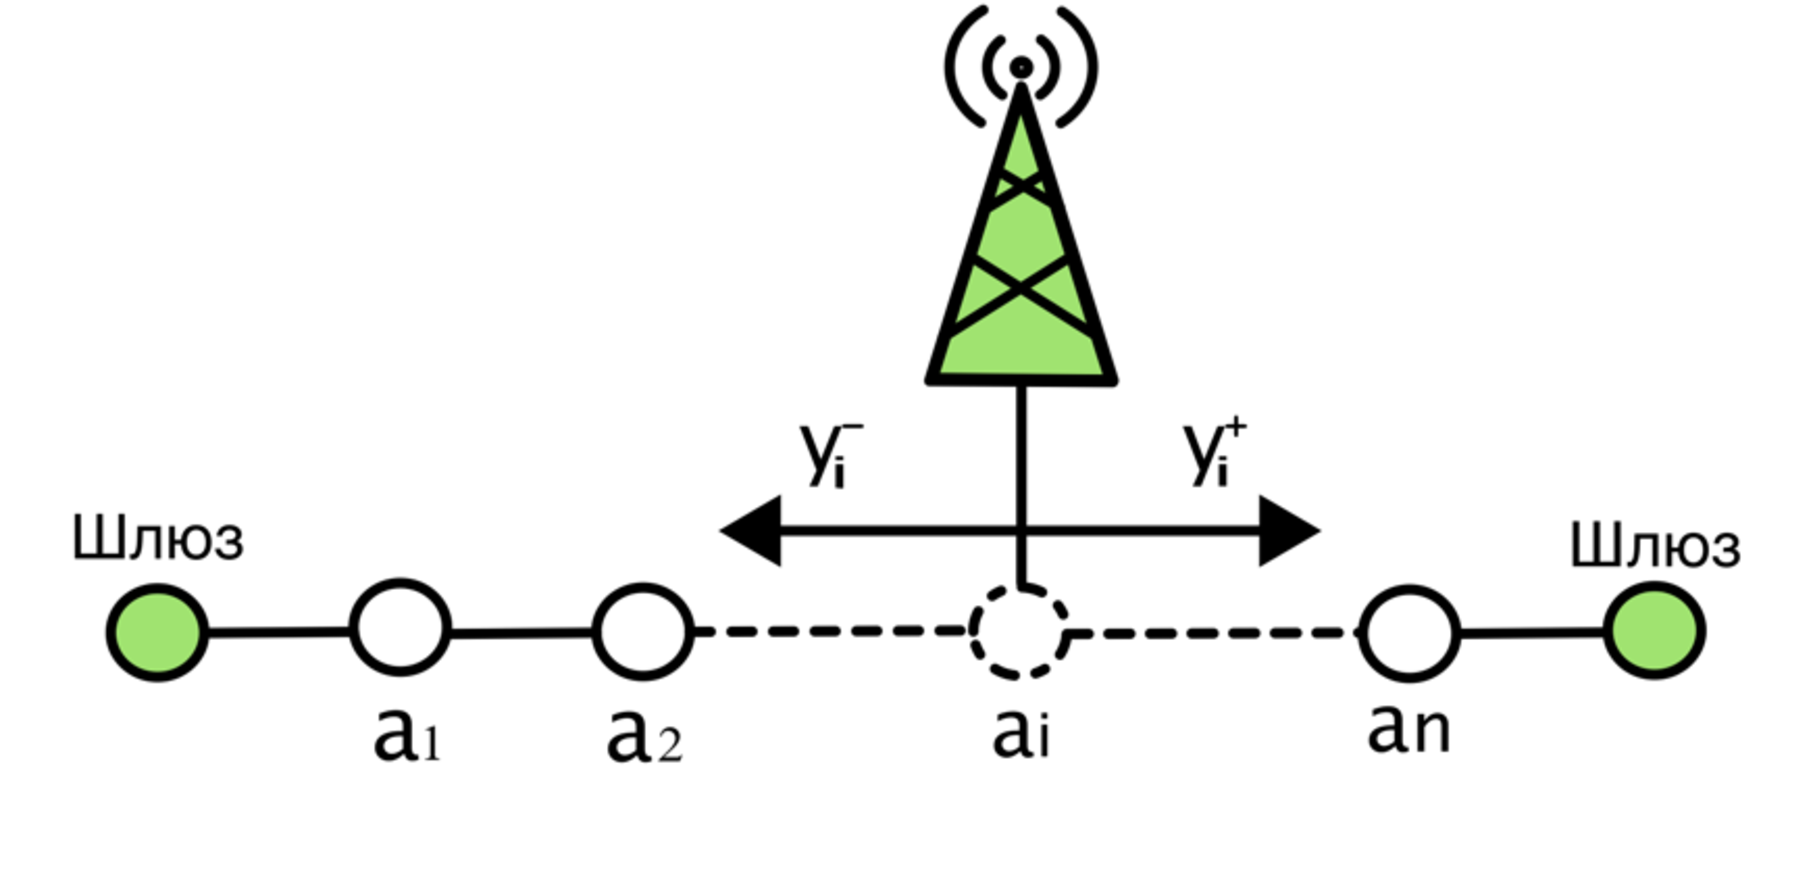
\includegraphics[scale=0.15]{station_coverage.pdf}}
        \center{\textbf{Охват покрытия станции}}
    \end{minipage}

    % \bigskip
    % \fontsize{8pt}{7.2}\selectfont
    % где $y_i^+$ и $y_i^-$ , $i= \overline{0,n+1}$ определяют охват покрытия (справа и слева, соответственно) станций.

\end{frame}

\begin{frame}
    \frametitle{задача ЦЛП}
    \begin{minipage}[t]{0.5\linewidth}
        \begin{equation}
            \label{eq:part3_ei}
            e_i =  \sum\limits_{j=1}^m x_{ij}, \quad i = \overline{1,n}. 
          \end{equation}
    \end{minipage}

    \begin{minipage}[t]{0.5\linewidth}
        % \fontsize{8pt}{7.2}\selectfont
        
    \bigskip
    \bigskip
    \bigskip
    Суммарное покрытие между двумя станциями не больше расстояния между ними.
          

    \end{minipage}
    \hfill
    \begin{minipage}[t]{0.47\linewidth}
        
        \center{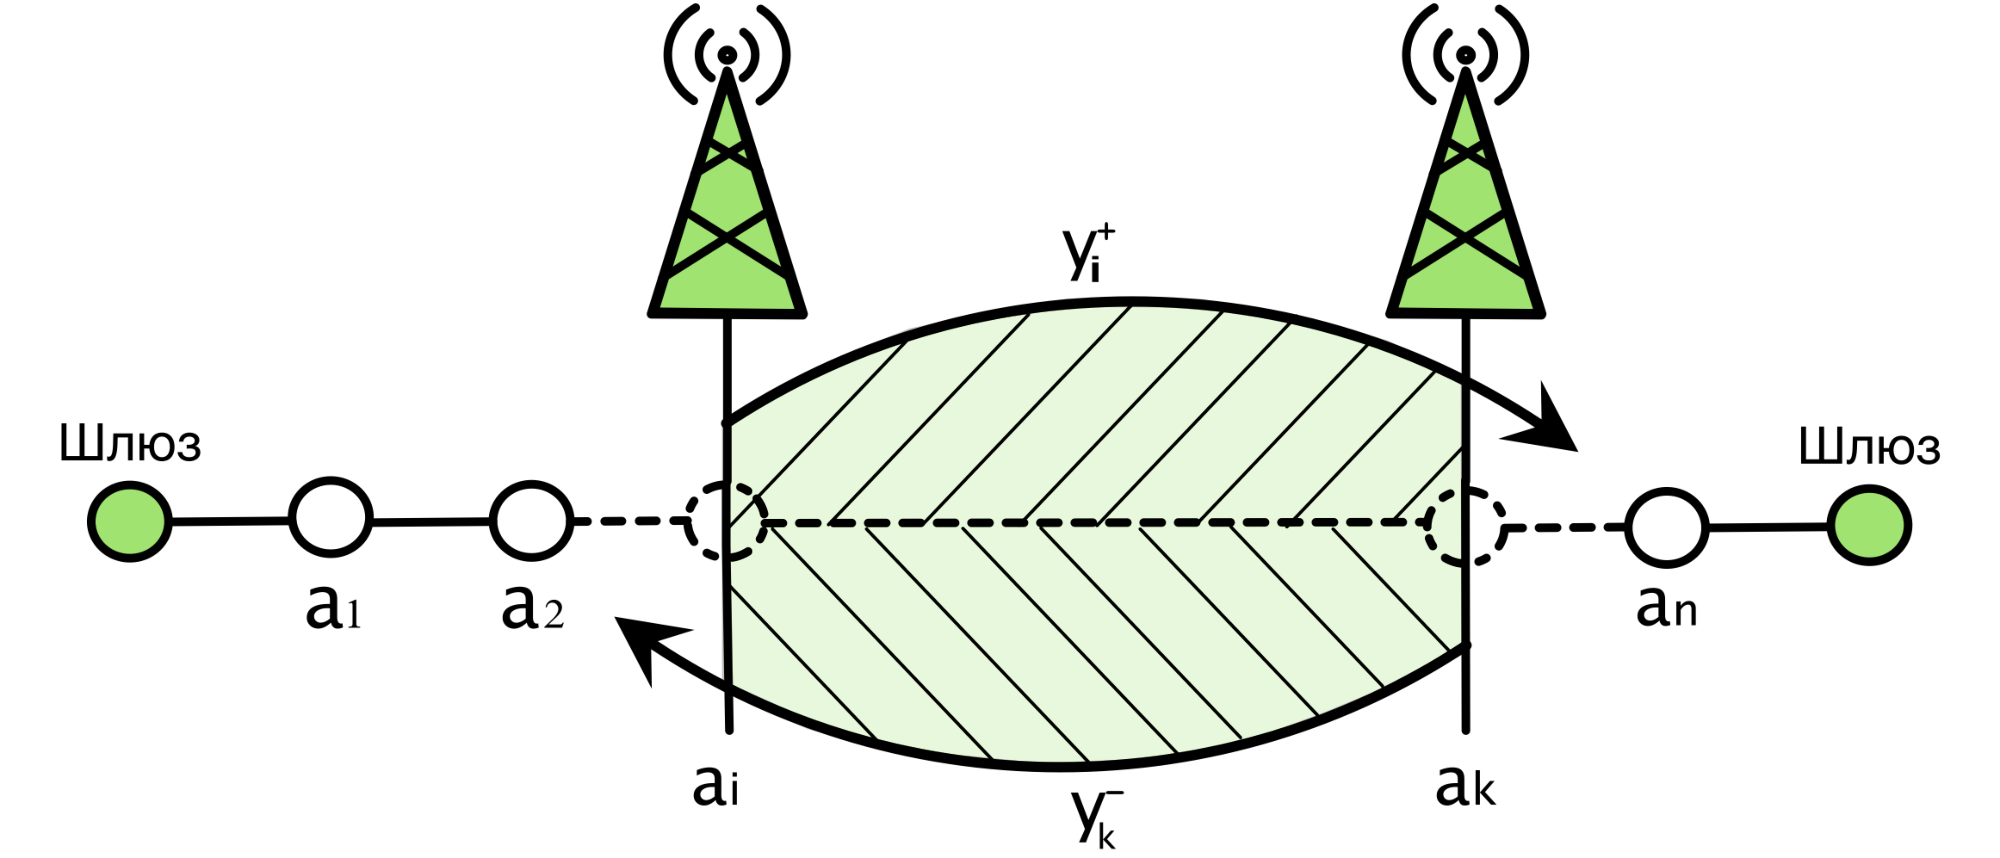
\includegraphics[scale=0.15]{total_coverage_between_points.pdf}}
        \center{\textbf{Покрытие между станциями}}
    \end{minipage}

    \bigskip
    \fontsize{8pt}{7.2}\selectfont
    \begin{equation}
        \label{eq:part3_yi_3}
        y_i^+ + y_k^- \leq \frac{l_k - l_i}{2} \cdot (e_i + e_k ) + (2 - e_i - e_k ) \cdot L, \quad i = \overline{1,n},  \quad k = \overline{i+1,n+1};
      \end{equation}
      
      \begin{equation}
        \label{eq:part3_yi_4}
        y_i^- + y_k^+  \leq \frac{l_i-l_k}{2} \cdot (e_i + e_k) + (2 - e_i - e_k) \cdot L, \quad i = \overline{1,n}, \quad k = \overline{i-1,0},
      \end{equation}

\end{frame}

\begin{frame}
    \frametitle{задача ЦЛП}
    \begin{minipage}[t]{1\linewidth}
        \fontsize{9pt}{7.2}\selectfont
        Введем переменные $z_{ijkq}, i = \overline{1,n}; j= \overline{1,m}; k=\overline{1,n},  k \neq i; q= \overline{1,m}, q \neq j$.
    \bigskip
    $$
    z_ {ijkq} = 
     \begin{cases}
       1& \text{, если в точке $ a_i $ размещена станция $ s_j $} \\
        & \text{и данная станция связана со станцией} \\
        & \text{$ s_q $, размещенная в точке $ a_k $;} \\
       0 & \text{, в противном случае.}
     \end{cases}
    $$
    \bigskip
    \end{minipage}
    
    \begin{minipage}[b]{0.5\linewidth}
        Важно обеспечить связь любой станции со шлюзами на концах участка через систему размещенных станций. 

    \end{minipage}
    \hfill
    \begin{minipage}[t]{0.47\linewidth}
        
        \center{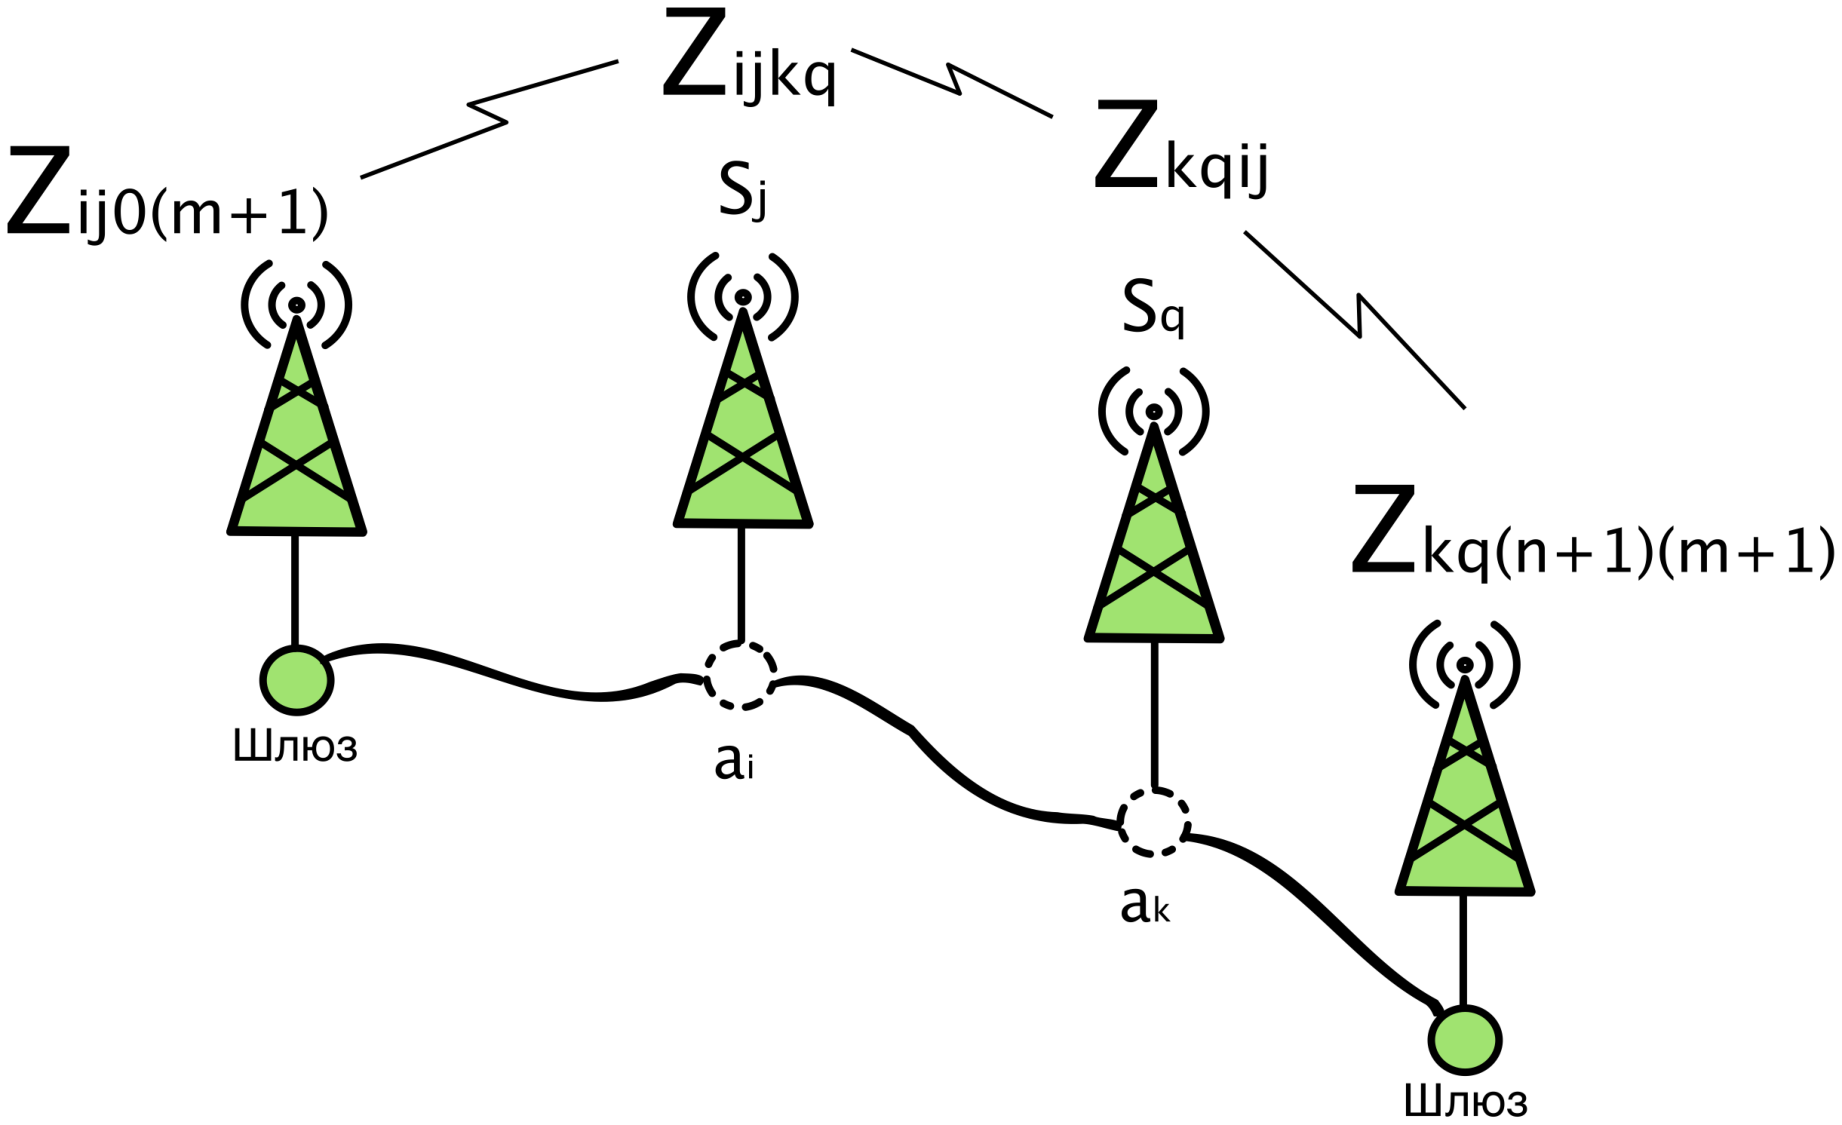
\includegraphics[scale=0.15]{station_link.pdf}}
        \center{\textbf{Связь между станциями}}
    \end{minipage}

\end{frame}


\begin{frame}[plain, noframenumbering]
    \frametitle{задача ЦЛП}
    
    \begin{minipage}[t]{0.99\linewidth}
        \fontsize{8 pt}{7.2}\selectfont
        \begin{equation}
            \label{eq:part3_z_ijkq_1}
            z_{ijkq} \leq e_i , \quad i = \overline{1, n}; \quad j = \overline{1, m}; \quad k = \overline{1,n}, k \neq i; \quad q = \overline{1,m}, q \neq j;
        \end{equation}
        
        
        \begin{equation}
            \label{eq:part3_z_ijkq_2}
            z_{ijkq} \leq e_k , \quad k = \overline{1, n}; \quad j = \overline{1, m}; \quad i = \overline{1,n}, i \neq k; \quad q = \overline{1,m}, q \neq j.
        \end{equation}
        
        
        \begin{equation}
            \label{eq:part3_z_ijkq_3_1}
            \sum\limits_{k=i+1}^{n} \sum\limits_{\substack{q = 1\\ q \neq j}}^m z_{ijkq} + z_{ij(n+1)(m+1)} = x_{ij} ,  \quad i = \overline{1, n}, \quad j = \overline{1, m}.
        \end{equation}

        
        \begin{equation}
            \label{eq:part3_z_ijkq_3_2}
            z_{nj(n+1)(m+1)} = x_{nj} \quad j = \overline{1, m}.
        \end{equation}

        
        \begin{equation}
            \label{eq:part3_z_ijkq_4_1}
            z_{1j0(m+1)}= x_{ij}, \quad j = \overline{1, m};
        \end{equation}

        
        \begin{equation}
            \label{eq:part3_z_ijkq_4_2}
            z_{ij0(m+1)} + \sum\limits_{k=1}^{i-1} \sum\limits_{\substack{q = 1\\ q \neq j}} z_{ijkq}= x_{ij}, \quad i = \overline{2, n}, \quad j = \overline{1, m}.
        \end{equation}

        
        \begin{equation}
            \label{eq:part3_z_ijkq_5}
            \sum\limits_{i=k+1}^{n} \sum\limits_{\substack{j=1 \\ j \neq q}}^m z_{ijkq} = x_{kq} , \quad k = \overline{1, n-1}, \quad q = \overline{1, m};
        \end{equation}

        
        \begin{equation}
            \label{eq:part3_z_ijkq_6}
            \sum\limits_{i=1}^{k} \sum\limits_{\substack{j=1 \\ j \neq q}}^m z_{ijkq} = x_{kq} , \quad k = \overline{2, n}, \quad q = \overline{1, m};
        \end{equation}
    \end{minipage}

\end{frame}


\begin{frame}
    \frametitle{задача ЦЛП}
    \begin{minipage}[t]{1\linewidth}
        \fontsize{6pt}{7.2}\selectfont
        $\forall i= \overline{1,n}$:
        \begin{equation}
          \label{eq:part3_z_ijkq_7}
          z_{ijkq}(R_{jq}-(a_i-a_k ))\geq 0, \quad k=\overline{0,i-1}; \quad j=\overline{1,m}; \quad q= \overline{1,m}, q \neq j; 
        \end{equation}
        
        \begin{equation}
          \label{eq:part3_z_ijkq_8}
          z_{ijkq} (R_{jq}-(a_k-a_i )) \geq 0, \quad k=\overline{i+1,n+1}; \quad j=\overline{1,m}; \quad q= \overline{1,m}, q \neq j.
        \end{equation}
    \bigskip
    \end{minipage}
    
    \begin{minipage}[и]{0.5\linewidth}
        \fontsize{8pt}{7.2}\selectfont
        Радиусы связи размещенных станций должнs быть не меньше расстояния между ними
        \bigskip
        \bigskip
        \bigskip

    \end{minipage}
    \hfill
    \begin{minipage}[b]{0.47\linewidth}
        
        \center{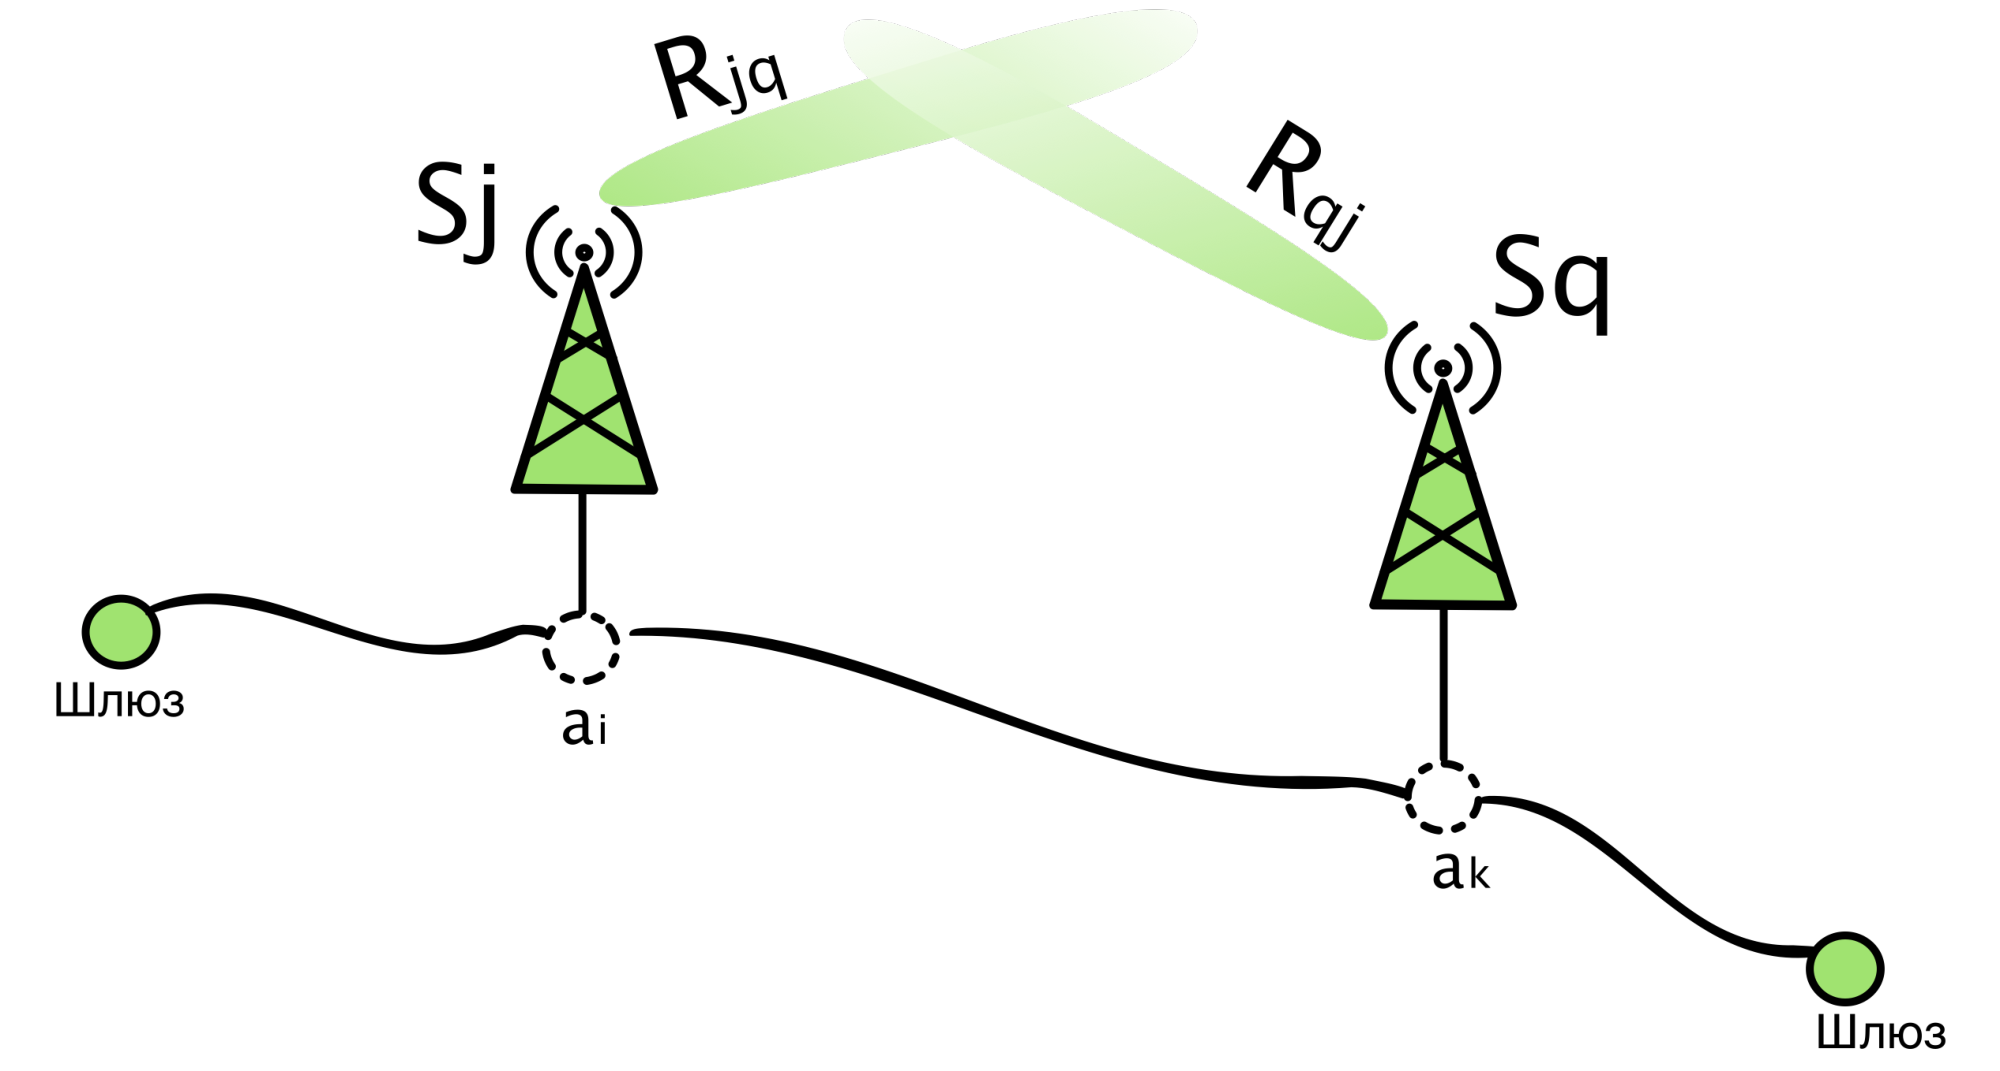
\includegraphics[scale=0.1]{station_link_between_points.pdf}}
        \center{\textbf{Обеспечение связи с соседней станцией}}
    \end{minipage}
    % \hfill
    \begin{minipage}[b]{0.99\linewidth}
        \fontsize{8pt}{7.2}\selectfont
        И бюджетное ограничение:

        \begin{equation}
        \label{eq:part3_cost}
        \sum\limits_{i=1}^n \sum\limits_{j=1}^m x_{ij} \cdot c_j \leq C.
        \end{equation}
    \end{minipage}

\end{frame}

\begin{frame}
    \frametitle{задача ЦЛП}
    
    
    Работа$^1$ содержит доказательство NP-полноты для частного случая задачи ЦЛП, когда вдоль линейной территории размещают множество однотипных станций с одинаковыми параметрами. 
    \bigskip
    
    Представленная в данном исследовании модель (1) - (18) рассматривает общий случай размещения, когда вдоль линейного участка размещают множество различных станций с разными техническими параметрами. Следовательно, данная задача является также NP-полной.
    \bigskip
    
    Представленная математическая модель рассчитывалась алгоритмом Лэнд и Дойг (1960).
    \bigskip

    \bigskip
    \bigskip
    \begin{minipage}[b]{0.99\linewidth}
        \fontsize{6pt}{7.2}\selectfont
    1. On a problem of base stations optimal placement in wirelessnetworks with linear topology. — [текст]. / — R. Ivanov [и др.] //Communications in Computer and Information Science. — 2018. —т. 919. — с. 505—513.
    \end{minipage}

\end{frame}

\begin{frame}
    \frametitle{Комбинаторная модель}
    Алгоритмы решения общего вида задач ЦЛП не учитывают специфику конкретной задачи.

    \bigskip
    Разработан специальный алгоритм размещения базовых станций \textbf{метода ветвей и границ (МВиГ)} для комбинаторной модели в экстремальной форме.

    \bigskip
    \textit{Допустимой расстановкой станций} назовем такой возрастающий по величине координат $l_i$  набор пар $P = \{a_i, s_j\},a_i \in A,i \neq 0,i \neq n+1;s_j \in S$.
    % \end{minipage}

\end{frame}

\begin{frame}
    \frametitle{Комбинаторная модель}
    Для каждой расстановки выполняются требования:

    \begin{enumerate}
        \item  для каждой пары $(a_i,s_j)$:
            \begin{itemize}
                \item слева: либо найдется такая пара $(a_k,s_q)$, что, $l_i - l_k \leqslant R_{jq}$  и $l_i - l_k  \leqslant R_{qj}$, либо $l_i-l_0 \leqslant R_{j0}$ и $l_i - l_0 \leqslant R_{0j}$;
                \item справа: либо найдется такая пара $(a_t,s_g)$, что, $l_t-l_i \leqslant R_{jq}$ и $l_t - l_i \leqslant R_{qj}$, либо $l_{n+1}-l_i \leqslant R_{j(m+1)}$ и $l_{n+1}-l_i \leqslant R_{(m+1)j}$. 
            \end{itemize}
    Данное требование гарантирует, что любая станция может быть связана со станциями на концах отрезка либо через промежуточные станции, либо непосредственно;
        \item в одной точке стоит не более одной станции;
        \item сумма задержек по всем размещенным станциям меньше заданной величины $T$ – средней межконцевой задержки по времени по всей системе станций;
        % \begin{displaymath}
        %     \label{eq:part3_e2e_delay}
        %     \sum\limits_{j \in S_\sigma} \overline{T_j} \leqslant T,
        % \end{displaymath}
    % где $S_\sigma$ – множество размещенных станций, $\overline{T_j}$ -- среднее время задержки на станции.
        \item суммарная стоимость размещенных станций меньше заданного бюджетного ограничения  $C$.
    \end{enumerate}

\end{frame}

\begin{frame}
    \frametitle{Комбинаторная модель}
    Каждой допустимой расстановке станций $P$ соответствует величина покрытия $z(P)$, определяемая как суммарная область покрытия станции, входящих в набор пар $P$.

    Для удобства описании в дальнейшем алгоритмов введем понятие «недопокрытия»:

    \begin{displaymath}
        f(P) = L - z(P)
    \end{displaymath} 

    \textbf{Задача 1.}
    Пусть $G$ -- множество всех допустимых расстановок $P$.

    \bigskip

    Тогда требуется найти такую допустимую расстановку  $P^*$, что
    \begin{displaymath}
        \label{eq:present_P}
        P^* = \argmin \limits_{P \in G} f(P)
    \end{displaymath}
\end{frame}

\begin{frame}
    \frametitle{Комбинаторная модель}
    \begin{minipage}[t]{1\linewidth}
        \fontsize{8pt}{7.2}\selectfont
        \textbf{Процедура построения бинарного дерева поиска} 
        \bigskip

        На каждой итерации, начиная с итерации $\nu=0$, разбиваем текущее подмножество $G_\nu$ на два подмножества $G^1_\nu$ и $G^2_\nu$. 
    \bigskip
    \end{minipage}
    
    \begin{minipage}[b]{0.5\linewidth}
        \fontsize{8pt}{7.2}\selectfont
        В качестве параметра разбиения воспользуемся переменной $\pi_{ij}$:

        \begin{itemize}
            \item $\pi_{ij}=1$, если наложено условие, что на месте $a_i$ расположена станция $s_j$;
            \item $\pi_{ij} = 0$, если наложено условие, что на месте $a_i$ станция $s_j$  располагаться не будет.
        \end{itemize}
        \bigskip

    \end{minipage}
    \hfill
    \begin{minipage}[b]{0.47\linewidth}
        
        \center{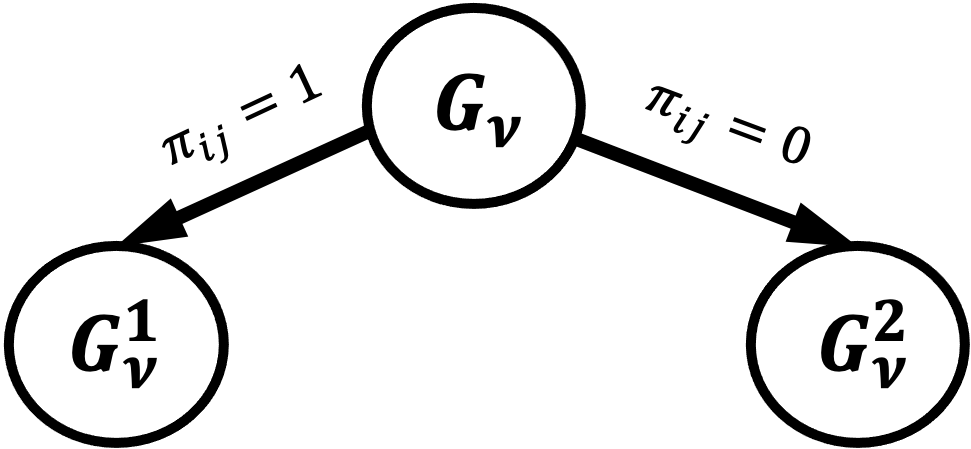
\includegraphics[scale=0.5]{binary_tree.png}}
        \center{\textbf{Узел бинарного дерева поиска}}
    \end{minipage}
    \hfill
    \begin{minipage}[b]{1\linewidth}
        \fontsize{8pt}{7.2}\selectfont
        \textbf{Алгоритм метода ветвей и границ.}
        \bigskip

        Для построения алгоритма МВиГ были разработаны методы исследования вершин дерева на возможность их закрытия.
        \bigskip

        В соответствии с техникой МВиГ закрытие вершины в результате исследования, соответствующего ей множества $G_\nu$ возможно \textbf{в трех случаях}:
    \end{minipage}

\end{frame}

\begin{frame}
    \frametitle{Комбинаторная модель}
    \underline{\textit{\textbf{Случай 1.}}} Множество $G_\nu$ -- пусто, т.е. доказано, что в множестве $G_\nu$ при данном наборе фиксированных и запрещенных переменных $\pi_{ij}$ нет ни одной допустимой расстановки $P$.
    \bigskip

    \underline{\textit{\textbf{Случай 2.}}} Доказано, что в множестве $G_\nu$ не может быть допустимой расстановки $P$ с меньшим значением целевой функции (19), чем у лучшей расстановки $\widehat{P}$ из уже найденных. Значение функции $f(\widehat{P})$ называется «рекордом», а расстановка $\widehat{P}$ -- «рекордным решением». В качестве начального рекорда принимается число заведомо большое искомого оптимального решения, например, $L$ – длина всего отрезка.
    \bigskip 
    
    \underline{\textit{\textbf{Случай 3.}}} Найдено оптимальное решение на множестве $G_\nu$.
    % Прежде чем рассмотреть эти три случая, запишем важное свойство любого множеств $G_\nu$, являющееся следствием принятого правила выбора свободной переменной для разбиения очередного множества $G_\nu$ при прямом шаге.

\end{frame}

\begin{frame}
    \frametitle{Комбинаторная модель}
    
    На каждом узле проводится оценка "недопокрытия"  в виде суммы

    \begin{displaymath}
        W\left(G_\nu\right) = w_1 + w_2. 
    \end{displaymath}

    \begin{itemize}
        \item $w_1 \left(G_\nu \right)$ -- сумма все частичных «недопокрытий» слева от точки размещения и величины радиуса покрытия, размещаемой станций;
        \item $w_2 \left(G_\nu \right)$ вычисляется «для недопокрытия» справа на части $\beta$ до конца всего отрезка (точки $a_{n+1}$).
    \end{itemize}
    Оценку $w_2 \left(G_\nu \right)$ получим релаксацией условий, определяющих допустимую расстановку станций на участке $\beta$. Найдем такое подмножество $S_\beta$ множества станций $S$, состоящее из еще не размещенных станций и дающее минимальное «недопокрытие» на участке $\beta$ при выполнении только условий 2) – 4). 
    
\end{frame}

\begin{frame}
    
    \frametitle{Комбинаторная модель}
    \fontsize{8pt}{7.2}\selectfont
    Для этого сформулируем следующую задачу булевого программирования.

    \underline{\textit{\textbf{Задача 2.}}}
    \begin{displaymath}\label{present:task2}
        z = |\beta| - \sum\limits_{x_j \in S_\beta} r_j x_j \rightarrow min.
    \end{displaymath}

    \begin{displaymath}\label{eq:part4_task2_cost}
        \sum\limits_{x_j \in S_\beta} c_j x_j \leqslant C,
    \end{displaymath}

    \begin{displaymath}\label{eq:part4_task2_m}
        \sum\limits_{x_j \in S_\beta} x_j \leqslant m,
    \end{displaymath}

    \begin{displaymath}
        x_j \in \{0, 1\},
    \end{displaymath}
    где $|\beta|$ -- длина отрезка отрезка  $\beta$, $m$ -- число свободных мест для размещения станций на отрезке $\beta$.

    \bigskip
    Эффективность использования оценки в методе ветвей и границ определяется точностью оценки и временем ее вычисления. \underline{\textit{\textbf{Задача 2}}} -- это задача ЦЛП, являющаяся труднорешаемой. 

    При снятии любого одного из ограничений \underline{\textit{\textbf{задача 2}}} представляет собой целочисленную задачу о ранце c эффективным псевдополиномиальным алгоритмом решения.
    % На основании \underline{\textit{\textbf{задачи 2}}} можно получить две оценки менее точные, но имеющие более эффективные методы решения. 
    
    % Заметим, что при снятии любого одного из ограничений \underline{\textit{\textbf{задача 2}}} представляет собой целочисленную задачу о ранце c эффективным псевдополиномиальным алгоритмом решения. При этом с точки зрения точности оценки, более перспективным представляется снятие ограничения на число свободных мест $m$, так как на практике, обычно, число возможных мест размещения станций существенно меньше числа размещенных станций, полученного в результате решения задачи. 
    \bigskip
    Если множество $G_\nu$ получено из материнского добавлением условия $\pi_{kt}=0$, то оценка $W(G_\nu)$ равна оценке материнского множества.

\end{frame}

\begin{frame}
    \fontsize{8pt}{7.2}\selectfont
    \frametitle{Комбинаторная модель}
    Если для найденной расстановки $P$ выполняются условия 1) – 4), которые для единственной расстановки легко проверяются, и

    \begin{displaymath}
        f(P) < f(\widehat{P}),
    \end{displaymath}
    то $f(P)$ принимается за новый рекорд $f(\widehat{P})$, расстановка $P$ становиться новым рекордным решением $\widehat{P}$ и выполняется шаг обратного хода по дереву поиска. Если неравенство не выполняется, то рекорд остается прежним и выполняется шаг обратного хода.

    \bigskip
    Работа алгоритма МВиГ заканчивается, когда все вершины дерева поиска закрыты, при этом решение задачи: 

    \begin{displaymath}
        P^{*} = \widehat{P},  f(P^*) = f(\widehat{P}).
    \end{displaymath}

    \bigskip
    \bigskip
    Обе задачи, в виде ЦЛП и в виде комбинаторной модели в экстремальной форме относятся к широкому к \textbf{классу задач размещения мощностей}. Отличительной особенностью рассмотренных задач является наличие условия на связь между размещаемыми объектами и линейная контролируемая территория.
\end{frame}

\begin{frame}
    \frametitle{Численный результат}

    Требуется разместить весь набор $m$ имеющихся однотипных станций. Множество всех возможных вариантов комбинаций $m$ станций на  $n$ местах запишем как $\Gamma$. Общее количество $\gamma \in \Gamma$:
    В МВиГ отпустим ограничение на межконцевую задержку.
    \begin{displaymath}
    \gamma = C_n^m \times m!.
    \end{displaymath} 
 
    Характеристика сравенения двух моделей --  \textbf{количество пройденных узлов} в ходе поиска оптимального значения.

    % В таблице показаны результаты решения задач для различного числа количества размещения и количества станций с использованием полного перебора, алгоритма МВиГ и модели ЦЛП. Для каждого набора станций и набора размещений были рассчитаны 10 примеров с различными числовыми входными данными. Для <<$-$>> решение задачи данной размерности методом полного перебора не было получено за 3 ч счета. 

    % Как видно из результов, представленных в таблице, при увеличении размерностей задачи, алгоритм МВиГ позволяет найти решение быстрее в ходе движения по дереву поиска.

    \begin{table}[b]\centering
        \caption{Результаты численного решения.}\label{tab:problems_BF_BnB_ILP}
        \begin{tabular}{|l|l|l|l|l|}
        \hline
        \textbf{Места} & \textbf{Станции} &	\textbf{Полный}& \textbf{МВиГ} & \textbf{ЦЛП} \\ 
        \textbf{размещения} &  &	\textbf{перебор}&  &  \\
        \hline
        7 &		5 &	17550  &	933 &		\textbf{753}\\
        9 &		5 &	71090  &	6478 &		\textbf{2669}\\
        10 &	5 &	126180 &	\textbf{1041} &		8551\\
        12 &	6 &	-- &		\textbf{8294} &		38569\\
        13 & 	6 &	-- &		\textbf{18485} &	30369\\
        \hline
        \end{tabular}
    \end{table}

\end{frame}

\begin{frame}
    \frametitle{Последовательность лучших решений}
    \fontsize{8pt}{7.2}\selectfont
    Рассмотрим \textbf{задачу 1.}

    \begin{displaymath}
        f(P^*) = min \{f(P), P \in G \}.
    \end{displaymath}

    Построим для этой задачи последовательность $\Gamma = P^1, P^2, ... ,P^k$ допустимых расстановок (решений) множества $G$ для заданного $k$, где 
    \begin{align}
        f(P^1) &= f(P^*), \nonumber  \\
        f(P^2) &= extr\{ f(P), P \in G \ P^1 \}, \nonumber \\
        ... \nonumber \\
        f(P^k) &= extr\{ f(P), P \in G \ P^1 \cup P^2 \cup ... P^k \}, \nonumber 
    \end{align} 
    
    Для итерационной процедура нахождения последовательности лучших решений достаточно неравенство $f(P) < f(\widehat{P})$ в алгоритме МВиГ заменить следующим неравенством 

    \begin{align}
        \label{eq:part4_is_less_than_record_d}
        f(P) \leqslant f(\widehat{P}) + d,
    \end{align}
    где $d = \varepsilon \cdot L > 0, \varepsilon$ -- заданное отклонение в процентах, и запоминать все рекорды, полученные в процессе решения задачи.

    % Увеличивая величину $d$, если при данном ее значении допустимого решения на этапе моделирования не найдено.
\end{frame}

\begin{frame}
    \frametitle{Выводы по Положению 1}
    \fontsize{8pt}{7.2}\selectfont

    \textbf{Представлены:}
    \begin{itemize}
        \item математическая модель ЦЛП;
        \item комбинаторная модель в экстремальной форме;
        \item алгоритм МВиГ для комбинаторной модели;
        \item итерационная процедура нахождения последовательности лучших решений.
    \end{itemize}

    \bigskip
    \textbf{Публикации:}
    \begin{minipage}[c]{1\linewidth}
        \fontsize{6pt}{7.2}\selectfont
        \begin{enumerate}
            \item \textit{Иванов,Р. Е.Задача оптимального размещения заданного множе­ства базовых станций беспроводной сети связи с линейной топо­логией [Текст] / Р. Е. Иванов, А. А. Мухтаров, О. Першин //Автоматизация, телемеханизация и связь в нефтяной промышлен­ности. — 2019. — Т. 549, No 4. — С. 39—45};
            
            \item \textit{Ivanov,R.A Problem of Optimal Location of Given Set of Base Sta­tions in Wireless Networks with Linear Topology[Текст]/ R. Ivanov,A. Mukhtarov, O. Pershin // Communications in Computer and Infor­mation Science. –– 2019. –– Vol. 1141 CCIS. –– P. 53––64. –– (Scopus,WoS)};
            
            \item \textit{Мухтаров,А. А.Математические  модели  задачи  размещениябазовых станций для контроля линейной территории [Текст] /А. А. Мухтаров, Р. Е. Иванов, О. Ю. Першин // Proceedings of the22nd International Scientific Conference on Distributed Computer andCommunication Networks: Control, Computation, Communications(DCCN-2019, Moscow). — 2019. — С. 205—212};
            
            \item \textit{On Optimal Placement of Base Stations in Wireless Broadband Net­works to Control a Linear Section with End-to-End Delay Limited[Текст]/ A. Mukhtarov [et al.] // Communications in Computer andInformation Science. –– 2020. –– Vol. 1337. –– P. 30––42};
            
            \item \textit{{Вишневский,В. М.Задача оптимального размещения базовыхстанций широкополосной сети для контроля линейной территориипри ограничении на величину межконцевой задержки [Текст] /В. М. Вишневский, А. А. Мухтаров, О. Першин // Материалы23-й Международной научной конференции "Распределенные ком­пьютерные и телекоммуникационные сети: управление, вычисление,связь"(DCCN-2020, Москва). — 2020. — С. 148—155}}.
        \end{enumerate}
    \end{minipage}

\end{frame}

\section{Положение 2}
\begin{frame}
    \begin{center}
        {Положение 2 - математические модели в виде задачи ЦЛП и экстремальной комбинаторной задачи для оптимального размещения базовых станций при проектировании БШС с линейной топологией}
    \end{center}
\end{frame}


\begin{frame}
    \frametitle{Разделяющие линии}
    \begin{minipage}[c]{0.47\linewidth}
        \center{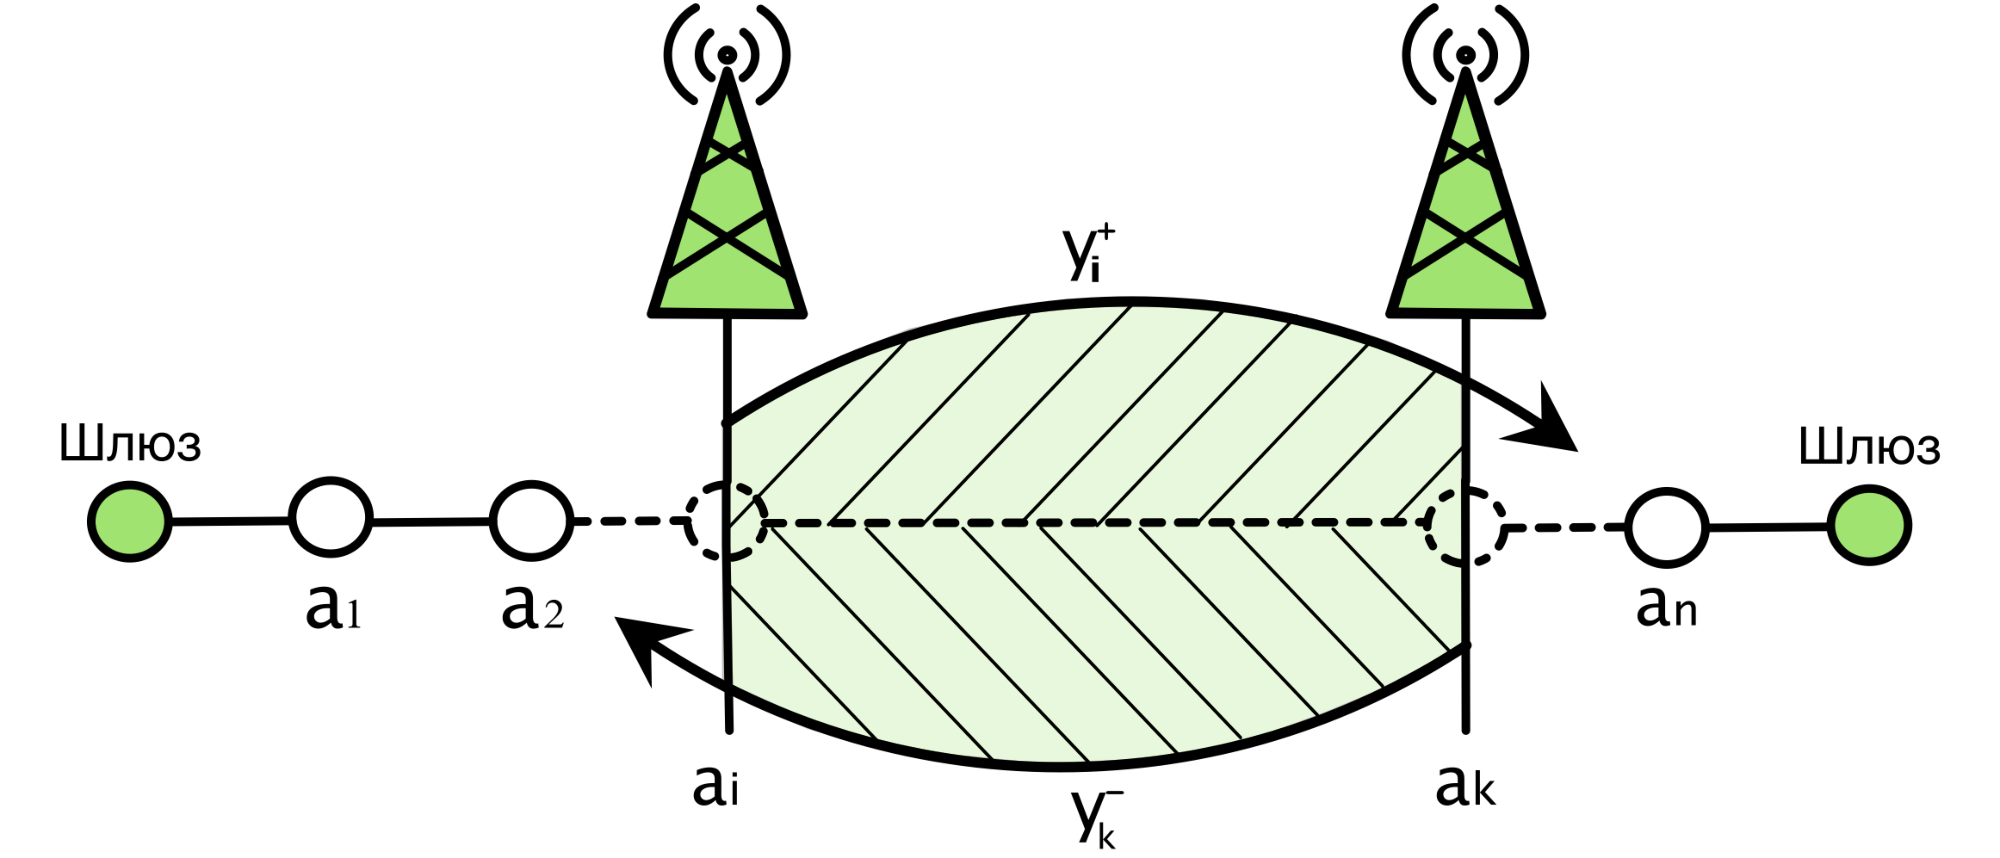
\includegraphics[scale=0.15]{total_coverage_between_points.pdf}}
        
        \bigskip
        \hrule{}
        \bigskip
        \textbf{Составная \\ подпись 1}
    \end{minipage}
    \hfill
    \vrule{}
    \hfill
    \begin{minipage}[c]{0.47\linewidth}
        \flushright
        \textbf{Составная \\ подпись 2}
        \center{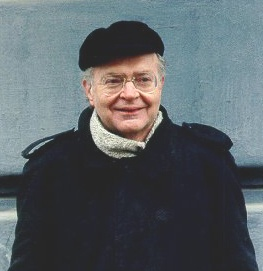
\includegraphics[width=1\linewidth]{knuth2}}
    \end{minipage}
\end{frame}

\begin{frame}

\end{frame}

\subsection{Нумерованные}

\begin{frame}
    \frametitle{Нумерованные списки}
    \begin{enumerate}
        \item один
        \item два
        \item три
    \end{enumerate}
\end{frame}
\note{
    Этот текст будет виден только если его отображение включено
    в~файле \textbf{Presentation/setup}.
    Для раздельного вывода презентации и заметок на~разные экраны (как
    в~impress или powerpoint) можно использовать программу
    \textit{pdf-presenter-console}.
}

\subsection{Не нумерованные}


\begin{frame}
    \frametitle{Перечисления}
    \begin{itemize}
        \item Проблема 1
        \item Проблема 2
        \item Проблема 3
    \end{itemize}
\end{frame}
\note[itemize]{
    \item Тезис 1
    \item Тезис 2
    \item Тезис 3
}

\subsection{Комбинированные}

\begin{frame}
    \frametitle{Комбинация списков}
    \begin{enumerate}
        \item \textbf{Задача 1}
              \begin{itemize}
                  \item Подзадача 1-1
                  \item Подзадача 1-2
              \end{itemize}
        \item \textbf{Задача 2}
              \begin{itemize}
                  \item Подзадача 2-1
                  \item Подзадача 2-2
                  \item Подзадача 2-3
              \end{itemize}
        \item \textbf{Задача 3}
              \begin{itemize}
                  \item Подзадача 3-1
                  \item Подзадача 3-2
                  \item Подзадача 3-3
              \end{itemize}
    \end{enumerate}
\end{frame}
\note[itemize]{
    \item Задача 1
    \item Задача 2
    \item Задача 3
}

\begin{frame}[allowframebreaks]
    \frametitle{Разделение слайда}
    Поясняющий текст
    \begin{itemize}
        \item Один
        \item Два
        \item Три
    \end{itemize}
    \framebreak
    Продолжение предыдущего слайда
\end{frame}

\section{Графика}
\begin{frame}[plain, noframenumbering]
    \begin{center}
        \Huge
        Графика
    \end{center}
\end{frame}


\begin{frame}
    \frametitle{Одиночное изображение}
    \centering
    
\includegraphics[width=0.8\linewidth]{latex} % окружение figure не требуется
\end{frame}

\begin{frame}
    \frametitle{Векторная графика}
    \begin{figure}
        \centering
        \ifdefmacro{\tikzsetnextfilename}{\tikzsetnextfilename{tikz_presentation}}{}% присваиваемое предкомпилированному pdf имя файла (не обязательно)
        \begin{tikzpicture}
  \draw[<->,thick] (0,6) -- (0,0) -- (10,0); % axis
  \draw[help lines] (3,0) -- (3,5); % fill end
  \draw[help lines] (6,0) -- (6,5); % flattop end
  \draw[help lines] (9,0) -- (9,5); % decay end
  \draw[<->, thin] (0,5) -- (3,5); % fill
  \draw[<->, thin] (3,5) -- (6,5); % flattop
  \draw[<->, thin] (6,5) -- (9,5); % decay
  \draw[blue, ultra thick] (0,0) -- (0,4) -- (6,4) -- (6,0); % power
  \draw[red, ultra thick, domain=0:3] plot (\x, {4*(1 - exp(-1.5*\x))}); % fill plot
  \draw[red, ultra thick, domain=3:6] plot (\x, {4*(1 - exp(-1.5*\x))}); % flattop plot
  \draw[red, ultra thick, domain=6:9.5] plot (\x, {4*(1 - exp(-9)) - 4*(1 - exp(-1.5*\x+9))}); % decay plot
  \node [above] at (0,6) {\(E_{acc}\)};
  \node [right] at (10,0) {\(t\)};
  \node at (1.5,5.4) {заполнение};
  \node at (4.5,5.4) {работа};
  \node at (7.5,5.4) {затухание};
  \node at (4.5,1.4) {пучки};
  \foreach \x in {3.1,3.3,...,5.9} {
    \draw[->, green, thick] (\x,0) -- (\x,1);
  }
\end{tikzpicture}
    \end{figure}
\end{frame}

\subsection{Расположение}

\begin{frame}
    \frametitle{Изображения по-вертикали}
    \centering
    \vfill
    
\includegraphics[width=0.8\linewidth,height=0.1\textheight]{latex} \\
    \TeX
    \vfill
    
\includegraphics[width=0.8\linewidth,height=0.2\textheight]{latex} \\
    \LaTeX
    \vfill
    
\includegraphics[scale=0.2]{latex} \\
    \vfill
\end{frame}


\begin{frame}
    \frametitle{Изображения по-горизонтали}
    \begin{minipage}[t]{0.47\linewidth}
        \textbf{Составная \\ подпись 1}
        \center{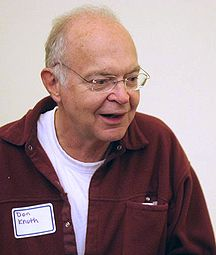
\includegraphics[width=1\linewidth]{knuth1}}
    \end{minipage}
    \hfill
    \begin{minipage}[t]{0.47\linewidth}
        \textbf{Составная \\ подпись 2}
        \center{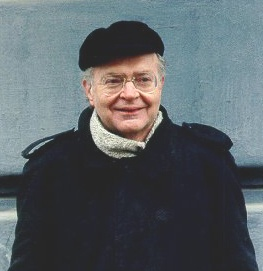
\includegraphics[width=1\linewidth]{knuth2}}
    \end{minipage}
\end{frame}

\subsection{Линии}

\begin{frame}
    \frametitle{Разделяющие линии}
    \begin{minipage}[c]{0.47\linewidth}
        \center{
\includegraphics[width=1\linewidth]{latex}}
        \bigskip
        \hrule{}
        \bigskip
        \textbf{Составная \\ подпись 1}
    \end{minipage}
    \hfill
    \vrule{}
    \hfill
    \begin{minipage}[c]{0.47\linewidth}
        \flushright
        \textbf{Составная \\ подпись 2}
        \center{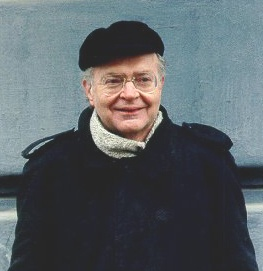
\includegraphics[width=1\linewidth]{knuth2}}
    \end{minipage}
\end{frame}

\section{Остальное}
\begin{frame}[plain, noframenumbering]
    \begin{center}
        \Huge
        Остальное
    \end{center}
\end{frame}

\subsection{Формулы}

\begin{frame}
    \frametitle{Формулы}
    \[
    \left\{
    \begin{array}{rl}
        \dot x = & \sigma (y-x)  \\
        \dot y = & x (r - z) - y \\
        \dot z = & xy - bz
    \end{array}
    \right.
    \]
\end{frame}

\begin{frame}
    \frametitle{amsmath}
    \centering
    \begin{minipage}[t]{0.5\linewidth}
        \begin{multline*}
            y = 1 x^1 + 2 x^2 + 3 x^3 + \\ + 4 x^4 + 5 x^5 + \dots
        \end{multline*}
    \end{minipage}
\end{frame}

\begin{frame}[allowframebreaks]
    \frametitle{Уравнения Максвелла}
    \centering{
        \small
        \def\arraystretch{1.8}%
        \begin{tabular}{ll}
            \toprule
            Интегральная форма                                                                                                                                            & Дифференциальная форма                                                          \\ \midrule
            \(Q_e(t) = \displaystyle\oiint_S \vec D(t) \cdot d\vec{s} = \displaystyle\iiint_V \rho_v(t) dv\)                                                              & \(\nabla \cdot \vec D(t) = \rho_v(t)\)                                          \\
            \(\displaystyle\oiint_S \vec B(t) \cdot d\vec{s} = 0\)                                                                                                        & \(\nabla \cdot \vec B(t) = 0\)                                                  \\
            \(V_{emf}(t) = \displaystyle\oint_L \vec E(t) \cdot d\vec{l}\) = \(- \displaystyle\iint_S \left[\frac{\partial\vec{B}(t)}{\partial t}\right] \cdot d\vec{s}\) & \(\nabla \times \vec E(t) = - \frac{\partial\vec{B}(t)}{\partial t}\)           \\
            \(I(t) = \displaystyle\oint_L \vec H(t) \cdot d\vec{l} = \displaystyle\iint_S \left[\vec J(t) + \frac{\partial\vec{D}(t)}{\partial t}\right] \cdot d\vec{s}\) & \(\nabla \times \vec H(t) = \vec J(t) + \frac{\partial\vec{D}(t)}{\partial t}\) \\ \midrule
            \(\displaystyle\oiint_S \vec J \cdot d\vec{s} = -\frac{\partial Q_e}{\partial t}\)                                                                            & \(\nabla \cdot \vec J = - \frac{\partial \rho_v}{\partial t}\)                  \\
            \bottomrule
            \multicolumn{2}{c}{\(\vec D(t) = \left[\varepsilon(t)\right] * \vec E(t)\)}                                                                                                                                                                     \\
            \multicolumn{2}{c}{\(\vec B(t) = \left[\mu(t)\right] * \vec H(t)\)}                                                                                                                                                                             \\
        \end{tabular}
    }
    \framebreak

    \hspace{0.05\linewidth}
    \centering{
        \small
        \def\arraystretch{1.8}%
        \begin{tabular}{ll}
            \toprule
            Интегральная форма                                                                                                                & Дифференциальная форма                               \\ \midrule
            \(Q_e = \displaystyle\oiint_S \vec D \cdot d\vec{s} = \displaystyle\iiint_V \rho_v dv\)                                           & \(\nabla \cdot \vec D = \rho_v\)                     \\
            \(\displaystyle\oiint_S \vec B \cdot d\vec{s} = 0\)                                                                               & \(\nabla \cdot \vec B = 0\)                          \\
            \(V_{emf} = \displaystyle\oint_L \vec E \cdot d\vec{l}\) = \(- \displaystyle\iint_S \left[j \omega \vec B\right] \cdot d\vec{s}\) & \(\nabla \times \vec E = - j \omega \vec B\)         \\
            \(I = \displaystyle\oint_L \vec H \cdot d\vec{l} = \displaystyle\iint_S \left[\vec J + j \omega \vec D\right] \cdot d\vec{s}\)    & \(\nabla \times \vec H = \vec J + j \omega \vec{D}\) \\ \midrule
            \(\displaystyle\oiint_S \vec J \cdot d\vec{s} = - j \omega Q_e\)                                                                  & \(\nabla \cdot \vec J = - j \omega \rho_v\)          \\
            \bottomrule
            \multicolumn{2}{c}{\(\vec D(t) = \left[\varepsilon\right] \vec E(t)\)}                                                                                                                   \\
            \multicolumn{2}{c}{\(\vec B(t) = \left[\mu\right] \vec H(t)\)}                                                                                                                           \\
        \end{tabular}
    }
\end{frame}

\subsection{Таблицы}

\begin{frame}
    \frametitle{Таблица}
    \centering
    \begin{tabular}{|l|l|}
        \hline
        \textbf{Заголовок 1} & \textbf{Заголовок 2} \\
        \hline
        Сумма                & \(b+a\)              \\
        \hline
        Разность             & \(a-b\)              \\
        \hline
        Произведение         & \(a*b\)              \\
        \hline
    \end{tabular}
\end{frame}

\begin{frame}
    \frametitle{Другая таблица}
    \centering
    \begin{tabular}{lc}
        \toprule
        \multicolumn{1}{c}{\textbf{Заголовок 1}} & \textbf{Заголовок 2} \\ \midrule
        Сумма                                    & \(b+a\)              \\
        Разность                                 & \(a-b\)              \\
        Произведение                             & \(a*b\)              \\
        \bottomrule
    \end{tabular}
\end{frame}


\subsection{Разное}

\begin{frame}
    \frametitle{Большой многоуровневый список}
    \begin{itemize}
        \item \textbf{Пункт 1}
              \begin{itemize}
                  \itemi Подпункт 1-1
                  \itemi Подпункт 1-2
              \end{itemize}
        \item \textbf{Пункт 2}
              \begin{itemize}
                  \itemi Подпункт 2-1
              \end{itemize}
        \item \textbf{Пункт 3}
              \begin{itemize}
                  \itemi Подпункт 3-1
                  \itemi Подпункт 3-2
              \end{itemize}
        \item \textbf{Пункт 4}
              \begin{itemize}
                  \itemi Подпункт 4-1
              \end{itemize}
        \item \textbf{Пункт 5}
              \begin{itemize}
                  \itemi Подпункт 5-1
                  \itemi Подпункт 5-2
                  \itemi Подпункт 5-3
              \end{itemize}
    \end{itemize}
\end{frame}

\begin{frame}
    \frametitle{Четыре изображения}
    \centering
    
\includegraphics[width=0.35\linewidth,angle=35]{latex}
    
\includegraphics[width=0.35\linewidth,angle=135]{latex}\\
    
\includegraphics[width=0.35\linewidth,angle=15]{latex}
    
\includegraphics[width=0.35\linewidth,angle=-15]{latex}
\end{frame}

